% Méthodes
\chapter{Matériels et Méthodes}
\section{Outils utilisés}

Voici la liste des outils utilisés pour le projet:
\begin{verbatim}
  - Ubuntu 24.04: L'OS utilisé pour le développement mais non nécessaire suite 
  à l'utilisation de Docker
  - Docker / Docker Compose: pour orchestrer l'environnement de développement
  - Redis: pour le stockage des données JSON en mémoire
  - MongoDB: pour la persistance des documents JSON
  - Python: pour le traitement des données et l'injection en base
  - Poetry: pour gérer les dépendances
  - LaTeX: pour la rédaction du rapport technique
  - VSCode: pour le developpement
  - Git: pour le contrôle de version
\end{verbatim}  
  

\subsubsection{Docker et Docker Compose}
Docker est utilisé pour orchestrer l’environnement de développement. 
Le fichier \texttt{compose.yaml} définit les services, incluant 
Redis, MongoDB et Python (Poetry). Chacun a son propre Dockerfile 
(ex.\@ \texttt{Dockerfile.redis}, \texttt{Dockerfile.mongo}). 
Cela garantit l’isolation des services, ce qui rend le projet facilement 
déployable sur différentes machines.

\subsubsection{Redis et Redis CLI}
Redis est utilisé comme base NoSQL pour le stockage des données JSON en mémoire. Les fichiers de connexion et de requêtes (\texttt{connectionRedis.py} et \texttt{requests\_redis.py}) gèrent l’interface entre l’API et Redis. Redis CLI est utilisé pour des tests rapides, et un fichier \texttt{.env.redis} gère la configuration sécurisée des variables d'environnement.
MongoDB est utilisé pour la persistance des documents JSON.\@ Il est intégré via PyMongo, avec des fichiers de connexion et de requêtes spécifiques (\texttt{connectionMongo.py} et \texttt{requests\_json.py}). Les données semi-structurées sont ainsi manipulées efficacement. Le fichier \texttt{Dockerfile.mongo} assure la configuration de MongoDB dans un conteneur.

\subsubsection{Python et Poetry}
Python est le langage principal pour le traitement des données et l’injection en base. Poetry est utilisé pour gérer les dépendances, avec un fichier \texttt{pyproject.toml} pour créer un environnement cohérent.

\subsection{Architecture du projet}

La figure \ref{fig:architecture} représentant l’architecture du projet avec Docker et bases NoSQL.\@ Cette architecture est basé sur un principe de séparation des résponsablitiés en séparant en différentes couches:

\begin{itemize}
  \item \textbf{API}: Cette couche communique avec la couche Services. Elle traîte les requetes HTTP (Get, Post, Put, Delete) et envoie les réponses en JSON
  \item \textbf{DAL}: Cette couche contient les fonctions de manipulation des données. Elle communique avec les bases de données via des connexions.
  \item \textbf{Services}: Cette couche contient les fonctions de traitement des données. Elle communique avec les bases de données via des connexions.
  \item \textbf{Config}: Cette couche contient les paramètres de configuration. Elle communique avec les bases de données via des connexions.
\end{itemize}

Cette architecture est bénifique car elle permet d'avoir un code propre, modulable et réutilisable. En effet, chaque couche peut être modifiée indépendamment, ce qui facilite la maintenance et le développement de l'application. Concernant les performances, la séparation des couches permet de réduire le temps de chargement des données, ce qui améliore la performance de l'application.

\begin{figure}[H]
  \centering
  \includegraphics[width=0.45\textwidth]{architecture.png}
  \caption{Architecture du projet avec Docker et bases NoSQL}
  \label{fig:architecture}
\end{figure}


\section{Stratégie de Migration de SQL vers NoSQL}
La base de données SQL originale se composait de plusieurs tables interconnectées qui suivaient un modèle relationnel strict. Cependant, ce modèle, bien que robuste pour certains cas d’utilisation, a montré ses limites dans la gestion des données dynamiques et évolutives. Cela nous a conduit à prendre la décision de passer à une architecture NoSQL, plus adaptée aux besoins actuels.

Le schéma suivant illustre la structure de la base SQL avant migration: 

\begin{figure}[H]
  \centering
  \includegraphics[width=0.8\textwidth]{schema.png}
  \caption{Schéma de la base SQL}
\end{figure}

\subsection{Étape 1:Regroupement des informations de Vols, Avions et Pilotes}

Dans le modèle SQL, pour récupérer toutes les informations d'un vol, il était nécessaire de joindre les tables `VOLS', `AVIONS' et `PILOTES', car chaque table stockait les données d'une entité spécifique. Par exemple, la table `VOLS' contenait les informations sur le vol, mais il fallait ensuite faire une jointure avec `AVIONS' pour connaître les détails de l'avion, et avec `PILOTES' pour obtenir les informations du pilote.

En NoSQL, nous avons choisi de regrouper toutes ces informations dans un seul document au sein de la collection `Vols`. Cette approche permet de conserver toutes les données pertinentes pour un vol dans un seul document JSON.\@

\begin{verbatim}
Vol = {
  _id : 'V001',
  VilleD : 'Paris',
  VilleA : 'New York',
  DateD : '2024-12-01',
  HD : '08:00',
  DateA : '2024-12-01',
  HA : '14:00',
  Avion : { ... },
  Pilote : { ... }
}
\end{verbatim}

Ce choix a été motivé par plusieurs raisons:
\begin{itemize}
  \item \textbf{Élimination des jointures}: En SQL, récupérer ces informations nécessitait de multiples jointures. En NoSQL, en regroupant ces informations dans un seul document, nous réduisons considérablement le coût des requêtes.
  \item \textbf{Accès optimisé aux données}: Toutes les données relatives à un vol, un avion et un pilote étant dans un seul document, cela permet un accès plus rapide et plus direct.
  \item \textbf{Regroupement logique}: Les informations sur les vols, les avions et les pilotes sont souvent interrogées ensemble, il est donc logique de les stocker ensemble.
\end{itemize}

\subsection{Étape 2:Intégration des Classes de Vols}

Dans la base SQL, les différentes classes de service (`Economy', `Business') étaient stockées dans une table séparée appelée `DEFCLASSES',\@ et elles étaient liées à la table `VOLS' par le numéro de vol. Cela nécessitait une jointure supplémentaire pour récupérer les informations des classes disponibles pour chaque vol.

Dans le modèle NoSQL, nous avons décidé d’inclure les classes disponibles directement dans une liste au sein du document `Vol`. Chaque élément de cette liste contient la classe (`Economy', `Business') ainsi que son coefficient de prix.

\begin{verbatim}
  /* Classes disponibles pour le vol */
  Classes : [
    {
      Classe : 'Economy',
      CoeffPrix : 1.0
    },
    {
      Classe : 'Business',
      CoeffPrix : 1.5
    }
  ]
\end{verbatim}

Ce choix s'explique par les avantages suivants:
\begin{itemize}
  \item \textbf{Simplification des requêtes}: En incluant les informations des classes directement dans le document `Vol', nous évitons d’avoir à effectuer une jointure supplémentaire pour les récupérer.
  \item \textbf{Centralisation des données du vol}: Toutes les informations pertinentes concernant un vol (y compris les classes de service) sont désormais disponibles en une seule requête.
  \item \textbf{Flexibilité du modèle NoSQL}: Le format JSON nous permet de structurer ces informations sous forme de liste, ce qui correspond bien à la nature dynamique des classes de vol, et permet d’ajouter facilement de nouvelles classes si nécessaire.
\end{itemize}

\subsection{Étape 3:Gestion des Clients}

Dans le modèle SQL, la table `CLIENTS' stockait des informations sur les clients, notamment leur nom, adresse, et autres coordonnées. Les champs d'adresse (numéro de rue, nom de rue, code postal, ville) étaient représentés par plusieurs colonnes.

Dans la structure NoSQL, nous avons décidé d'imbriquer les informations d'adresse dans un sous-document appelé `Adresse' pour chaque document `Client'.

\begin{verbatim}
Client = {
  _id : 789,
  NomCl : 'Alice Dupont',
  Adresse : { ... },
  Email : 'alice.dupont@example.com',
  Telephone : '0123456789'
}
\end{verbatim}

Ce choix a été fait pour les raisons suivantes:
\begin{itemize}
  \item \textbf{Regroupement logique des informations}: En imbriquant les informations d'adresse dans un sous-document, nous améliorons la cohérence et la gestion des données.
  \item \textbf{Flexibilité}: Si des champs supplémentaires liés à l’adresse sont nécessaires à l’avenir (comme le pays ou la région), ils peuvent être ajoutés sans avoir à modifier toute la structure.
\end{itemize}

\subsection{Étape 4:Représentation des Réservations}

Dans la base SQL, la table `RESERVATIONS' établissait des relations entre les clients et les vols via des clés étrangères, reliant également les classes de service. Dans le modèle NoSQL, nous avons conservé ce concept de relation en utilisant des identifiants (`VolId' et `ClientId') pour relier les documents `Reservation' aux documents `Vol' et `Client'.

\begin{verbatim}
Reservation = {
  _id : 'R001',
  VolId : 'V001',
  ClientId : 789,
  NbPlaces : 2,
  Classe : 'Economy'
}
\end{verbatim}

Nous avons fait ce choix pour les raisons suivantes:
\begin{itemize}
  \item \textbf{Conservation des relations critiques}: Même dans un modèle NoSQL, certaines relations doivent être maintenues. Ici, nous utilisons des identifiants pour lier les réservations aux vols et aux clients sans dupliquer inutilement les données.
  \item \textbf{Économie de stockage}: En stockant uniquement les références aux documents `Vol' et `Client', nous évitons de dupliquer les informations des vols et des clients dans chaque réservation.
\end{itemize}

\section{Conversion des données TXT en JSON}

Le script~\ref{ann:code_json} montre la création de 3 documents json a partir de nos 6 tables, ces tables peuveut être intégré facilement à Redis en ayant comme index le nom de la collection et indice (id) et pour mongo cela peut être représenté en trois collections chacune avec ses documents.\@ et chaque document a un id unique.

\subsection{Insertion des documents dans Redis}

Pour insérer les documents dans Redis nous utiliserons le script~\ref{ann:redis_insert} qui charge les données JSON, les insère dans Redis et affiche un message de succès.

la figure \ref{fig:redis_insert} représente la sortie de la commande \texttt{redis-cli} qui affiche les données insérées dans Redis.

\begin{figure}[H]
  \centering
  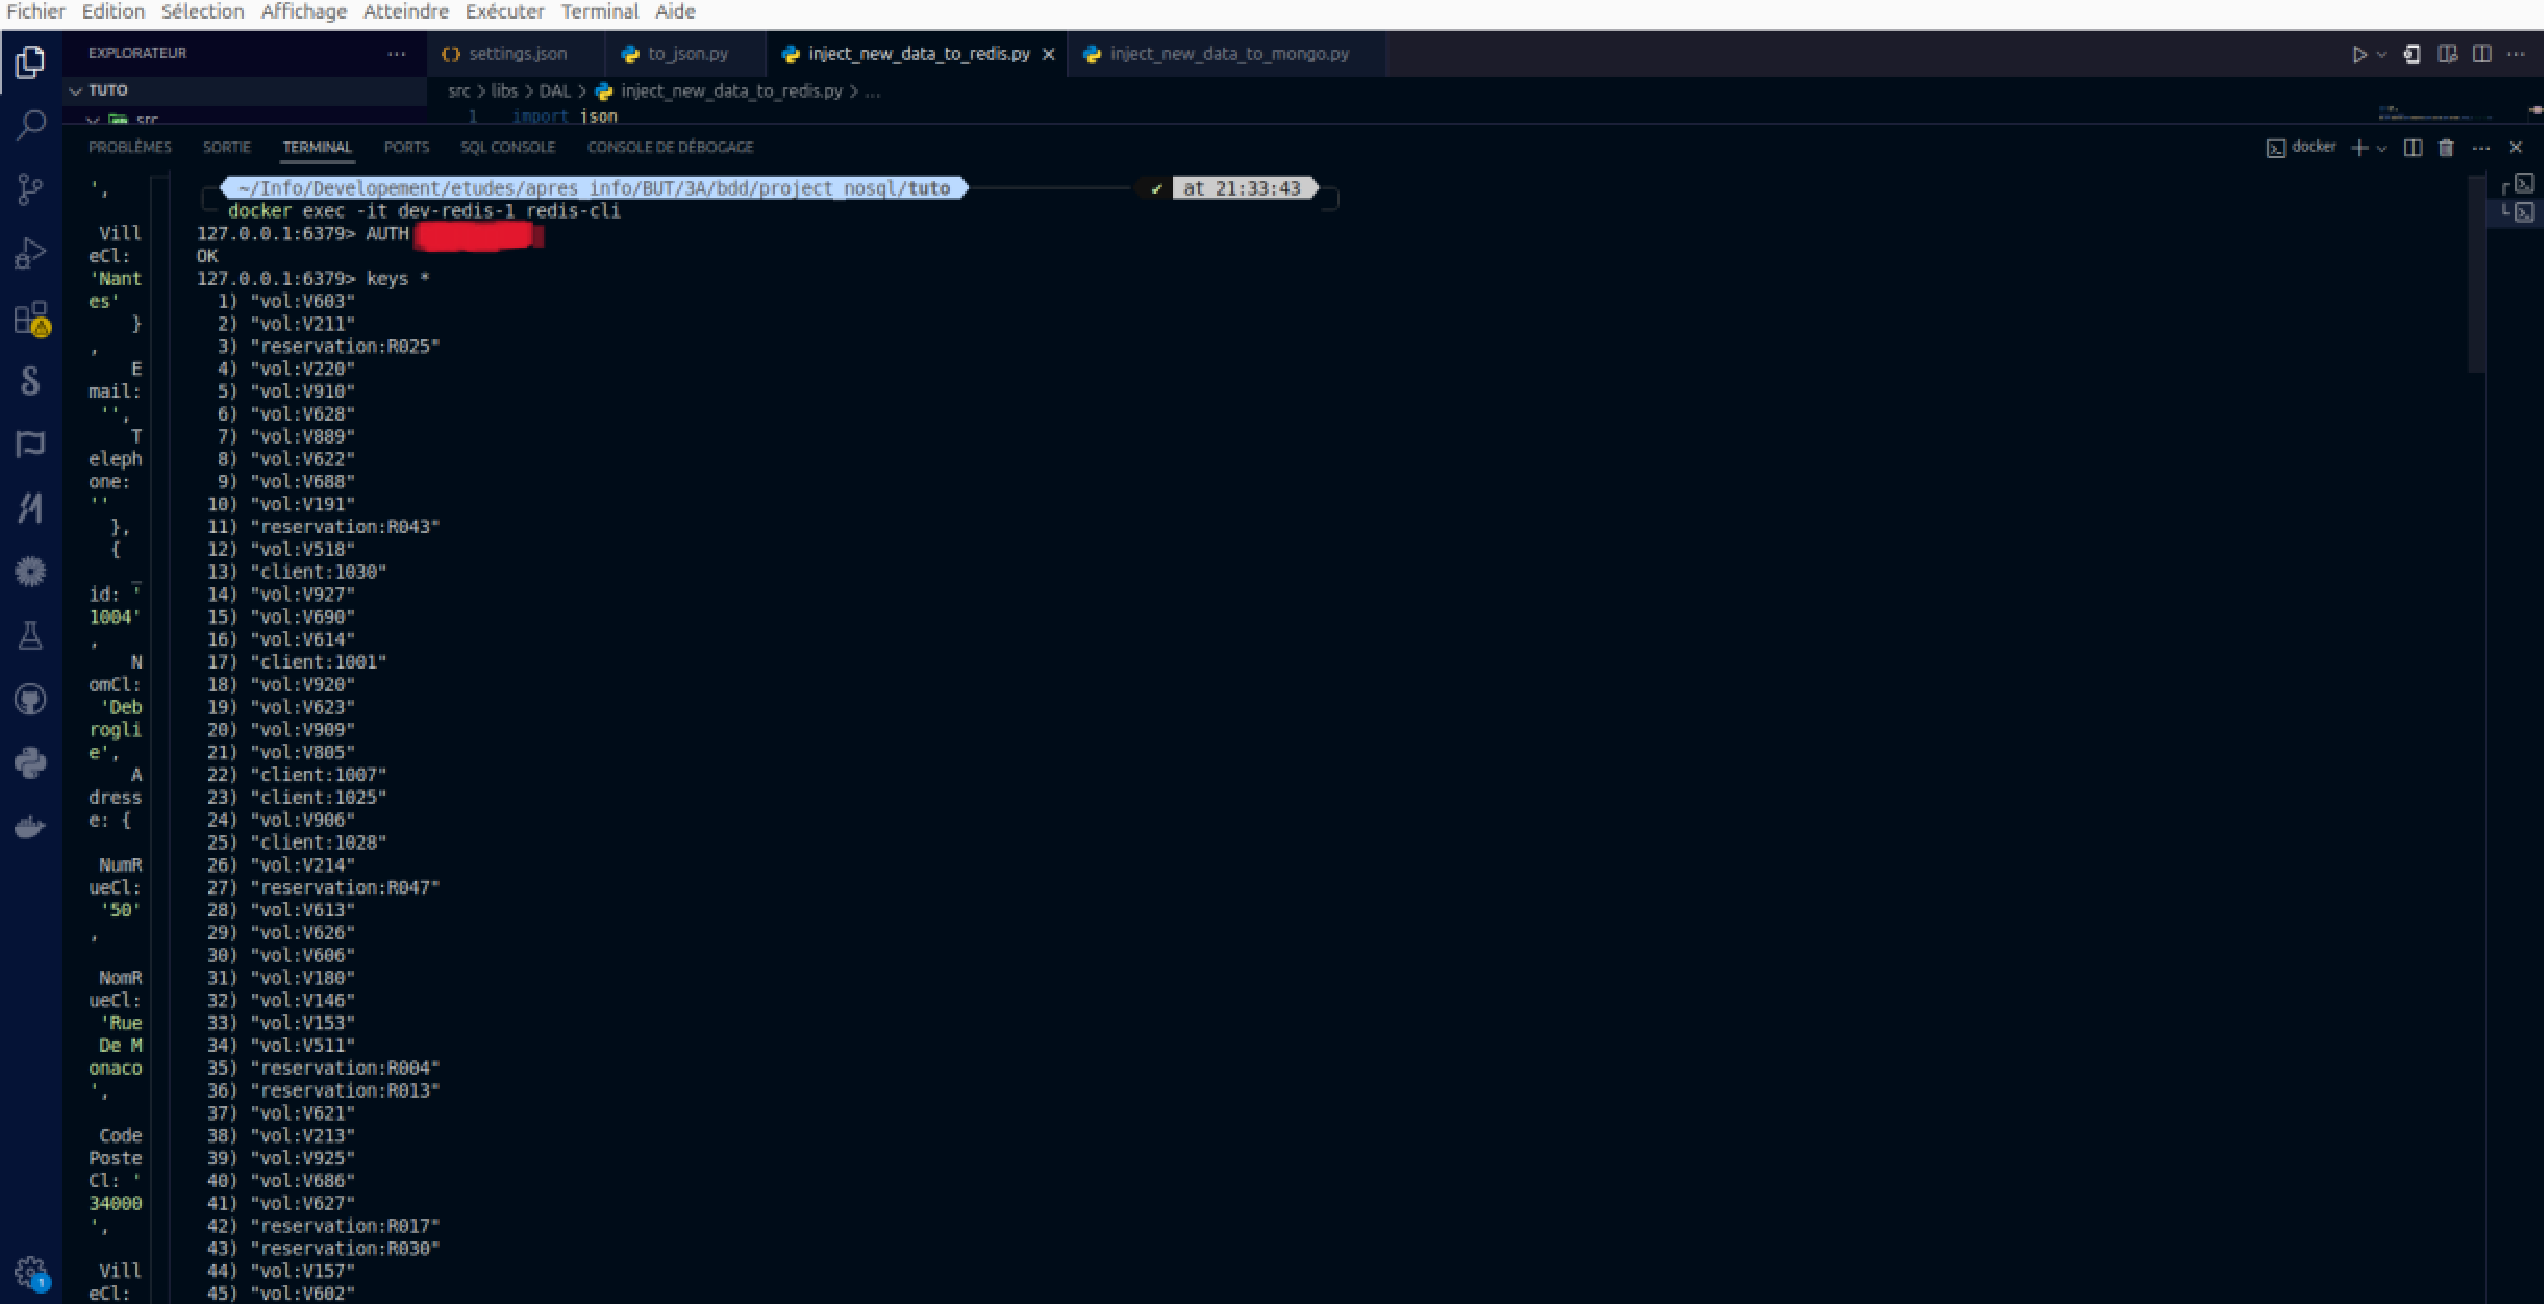
\includegraphics[width=1\textwidth]{redis.pdf}
  \caption{Insertion des documents dans Redis}
  \label{fig:redis_insert}
\end{figure}

\subsection{Insertion des documents dans MongoDB}

Pour insérer les documents dans MongoDB nous utiliserons le script~\ref{ann:mongo_insert} qui charge les données JSON, les insère dans MongoDB et affiche un message de succès.

la figure~\ref{fig:mongo_insert} représente la sortie de la commande \texttt{mongo} qui affiche les données insérées dans MongoDB.\@

\begin{figure}[H]
  \centering
  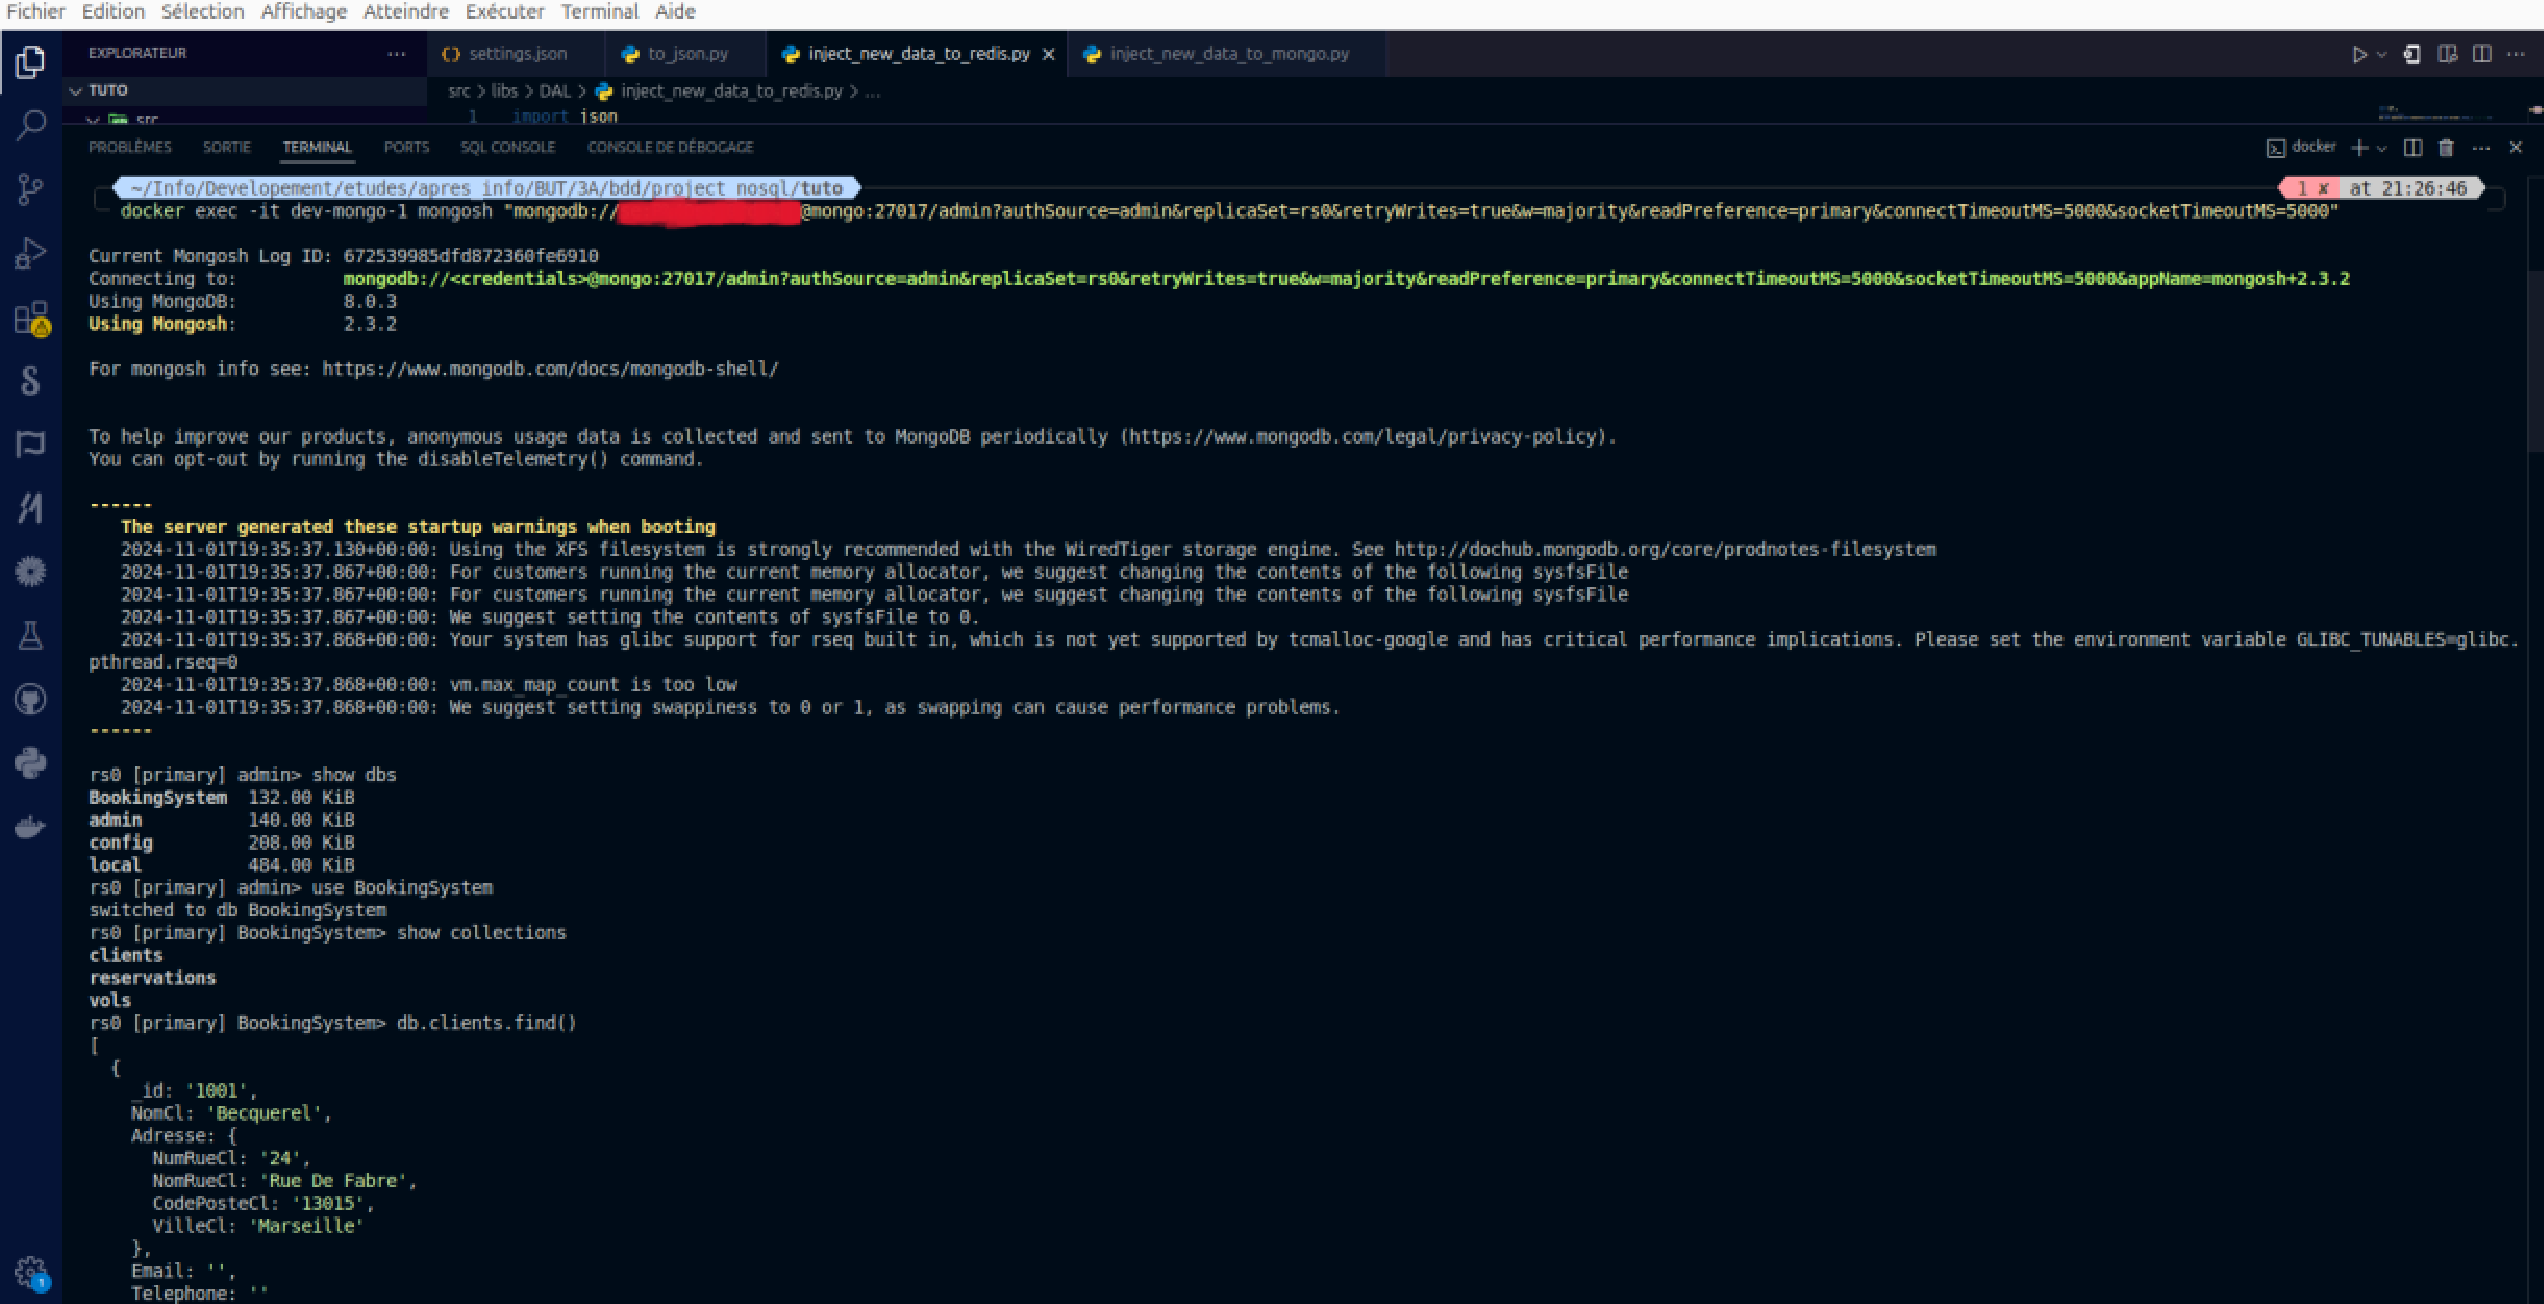
\includegraphics[width=1\textwidth]{mongo.pdf}
  \caption{Insertion des documents dans MongoDB}
  \label{fig:mongo_insert}
\end{figure}